%% 卒業論文概要原稿用テンプレート
\documentclass[onecolumn]{jsarticle}
%% パッケージの設定
\usepackage[dvipdfmx]{graphicx}
\usepackage{mseproc}
\usepackage{amssymb,amsmath}
\usepackage{bm}
\usepackage{url}

%% 学科名・発表番号
\renewcommand{\mplab}{ロボティックライフサポート研究室}
\renewcommand{\mpcode}{III--10}
%% 和文題目
\renewcommand{\mpjtitle}{
  卒業論文概要原稿用\LaTeXe テンプレート
}
%% 指導教員名・学籍番号・著者名
\renewcommand{\mpsupervisor}{東京~太郎~教授,都市~次郎~准教授}
\renewcommand{\mpsid}{1081200}
\renewcommand{\mpauthor}{山田~遥斗}

\begin{document}
\btitle
\section{このテンプレートについてa}
このファイル\texttt{bachelorFinal.tex}は,
東京都市大学工学部機械システム工学科の
卒業論文概要原稿を\LaTeXe で作成するためのテンプレートである.
基本事項はすべて,Word~2010のテンプレート\cite{msetemplateB}
を参照し,\LaTeXe で作成する場合の書式のみを本テンプレートに
合わせること.


\section{使用するための前提条件}
使用条件として下記を前提としている.
\begin{enumerate}
\item \LaTeXe にある程度習熟している\cite{Okumura2000}.
\item \pLaTeXe がインストールされている(\ref{sec:latexinstall}節参照).
\item \texttt{jsarticle.cls}がインストールされている\cite{Okumura2000}.
\end{enumerate}
テンプレート作成と動作確認はUbuntu~10.04上で実施した.
文字コードがEUCとなっているため,
Windows系OS上での利用の際は,Shift-JIS版を利用すること.

また,このファイルと一緒に配布しているスタイルファイルの
\texttt{mseproc.sty}が同じフォルダに存在する必要がある.
以下では,バックスラッシュ記号\verb+\+と
円マーク記号(半角の¥)は同一である.


\section{テンプレートの使用方法}
まずプリアンブル
\footnote{\verb+\begin{document}+の前}
の下記項目を注意深く設定する.

\subsection{研究室名・論文番号}
左上に所属研究室名と論文番号を表記するため,
\verb+\renewcommand{\mplab}{研究室名}+,\\
\verb+\renewcommand{\mpcode}{III--10}+ \\
をTable~\ref{table:lablist}に従って適当に書き変える.
%
\begin{table}[ht]
  \centering
  \caption{Lab. list in our department.}
  \label{table:lablist}
  \begin{tabular}{|l|l|}\hline
    I & 熱流体システム研究室 \\ \hline 
    II & 高機能機械制御研究室 \\ \hline
    III & ロボティックライフサポート研究室 \\ \hline 
    IV & 強度設計システム研究室 \\ \hline
    V & 計測電機制御研究室 \\ \hline
    VI & 宇宙システム研究室 \\ \hline
  \end{tabular}
\end{table}

\LaTeX のハイフンは\verb+-+を2個続けて書く(\verb+--+)ことに注意する.

\subsection{論文題目}
\verb+\renewcommand{\mpjtitle}{...}+
を設定する.

\subsection{指導教員名}
\verb+\renewcommand{\mpsupervisor}{...}+ \\
を設定する.

\subsection{学籍番号}
\verb+\renewcommand{\mpsid}{...}+
を設定する.

\subsection{著者名}
\verb+\renewcommand{\mpauthor}{...}+
を設定する.

\subsection{タイトル部の表示}
ここまで説明してきた上記の項目をプリアンブル設定した後に
\verb+\begin{document}+の後で\verb+\btitle+
を設定すれば,フォーマットに合わせたタイトル部が表示される.

\subsection{本文の記述}
上記を確認したら\texttt{bachelorFinal.tex}を適宜編集すればよい.


\section{利用上の注意}

\subsection{\texttt{jsarticle.cls}について}
このテンプレートを作者が意図した通りに利用するためには,
\texttt{jsarticle.cls}\cite{Okumura2000}が必要であり,その仕様に依存する.
したがって,\texttt{jsarticle.cls}のバージョンが違う場合は結果が
多少異なる可能性があるので注意する必要がある.また,
文字のデフォルトの大きさを変更しないように強く奨める.
例えば12ptに変更すると,\verb+\hspace*{10mm}+が12~mmの空白になる.

\subsection{PDFファイルへの変換について}
本年度の原稿提出はPDFファイルで行う.
写真などにビットマップイメージを用いている場合は
最終版の解像度に注意すること.
PDFへの変換方法は\ref{dvipdf}節で簡単に述べるが,詳細は
文献\cite{Kagi,TeXWiki}などを参照すること.
WinShellなどの統合環境ではメニューに用意されていることが多い.
PDFを作成した段階で専攻が指定する書式に適合しているかを最終確認すること.


\section{環境構築}
\label{sec:latexinstall}
Windows XP上での環境構築の指針を示す.

\subsection{\LaTeXe インストール}
\subsubsection{TeXインストーラ3}
「TeXインストーラ3」\cite{texinstaller}を用いると
一通りのソフトウエアを自動的にインストール・設定できる.
Plug-inを導入することでWinShellのインストールと環境設定も
行うことができる.
インストール時にブロードバンド環境を必要とする.
\subsubsection{美文書作成入門付属のCDを用いる}
文献\cite{Okumura2000}に付属のCDで一通りインストールできるが,
最新版ではないこともある.

\subsection{エディタや統合環境}
\subsubsection{\texttt{Winshell}}
\texttt{Winshell 3}をインストールすればGUIの統合環境を構築できる
\cite{TeXWiki}.
美文書作成入門\cite{Okumura2000}のCDにも入っているが最新版ではない
可能性がある.
\subsubsection{\texttt{Akasha}}
シェアウエアの使いやすいGUI統合環境.文献\cite{TeXWiki}のTeX用エディタを参照.
\subsubsection{\texttt{サクラエディタ}}
評判の良いエディタ.文献\cite{TeXWiki}を参照.
\subsubsection{\texttt{Meadow/Emacs+AUCTeX/YaTeX}}
有名なエディタと\LaTeXe の入力支援環境.マウスを使わずに
タイプセットできる.

\subsection{PDFへの変換}
\label{dvipdf}
texファイルをタイプセットして作成したdviファイルは下記の方法で
PDFファイルに変換できる.2番目以降はコマンドプロンプトの操作を
必要とする.
\subsubsection{統合環境}
WinshellやAkashaなどの統合環境の多くはPDFへの変換メニューを用意している.
\subsubsection{\texttt{dvipdfmx}}
dviからpdfに変換する.詳しくは文献\cite{TeXWiki}を参照.
\subsubsection{Adobe Acrobat}
まず\texttt{dvipsk}を用いてPSファイルに変換する.
\begin{verbatim}
  > divpsk -Ppdf -t a4 xxx.dvi
\end{verbatim}
次にAdobe AcrobatでPDFファイルに変換する
\footnote{Acrobat Elements以上で変換できる.Adobe Readerでは変換できない.}
.文献\cite{TeXWiki}を参照すること.


\section{数式の書き方}

\subsection{数式の記述に関する注意}
式には番号をつける.
\begin{equation}
  \bm{M} \ddot{\bm{q}} + \bm{C}(\bm{q},\dot{\bm{q}}) 
  + \bm{D} \dot{\bm{q}} + \bm{G}(\bm{q}) = \bm{\tau}
  \label{eqn:manipulatoreqs}
\end{equation}
式を並べる場合は次のようにする.
\begin{eqnarray}
  \dot x & = & A x + B u \\
  y & = & C x + D u
\end{eqnarray}

\subsection{数式の参照}
上の最初の方程式を参照するには,\verb+\ref+を用いて
(\ref{eqn:manipulatoreqs})とする.

\subsection{文章中の数式の記述}
文章中に数式を書く場合は,p=0 ではなく,\verb+$p=0$+と書いて
$p=0$と出力する.
分数を書く場合には,$\frac{y}{x}$ ではなく,$y/x$とする.

\subsection{三角関数など}
\verb+$sin$+と書くと,$s\times i\times n$の意味の$sin$となってしまう.
\verb+$\sin$+と書けば,$\sin$と正しく出力される.他にも
$\cos$,$\tan$,$\log$など一般的な数学関数はコマンドが用意されている.


\section{表の書き方}
表を書く場合には,Table~\ref{table:jitter}のようにする.
\begin{table}[ht]
  \centering
  \caption{Scheduling jitter data.}
  \label{table:jitter}
  \begin{tabular}{|c|c|c|}\hline
    & Maximum [$\mu$s] & Average [$\mu$s] \\ \hline \hline
    Standard kernel & $2.06 \times 10^3$ & $1.45 \times 10^3$ \\ \hline
    Real-time kernel & 92.0 & 25.5 \\ \hline
  \end{tabular}
\end{table}


\section{図の取り込み}
\TeX 文書に挿入する図のファイル形式は通常EPSファイルを用いる.

\subsection{図の記述}
図の幅の指定値は最大で80~mmとする.
長さ変数の\verb+\figurewidth+を用意してある.
これを用いると自動的にcolumnの幅いっぱいに表示される.例:\\
{\small \verb+\includegraphics[width=\figurewidth,clip]{...}+}

図中の語句やキャプションは必ず英語で記述する.

\subsection{図の参照の例}
Fig.~\ref{fig:snapthru}は2次遅れ系
%
\begin{equation}
  \frac{Y(s)}{U(s)} = \frac{K\omega_n^2}{s^2+2\zeta \omega_n s + \omega_n^2}
\end{equation}
%
について,$K=\omega_n=1$の下で減衰係数$\zeta$を
$\zeta=2,1, 0.8, 0.6, 0.4, 0.2, 0$とした場合の単位ステップ応答
波形である.
%
\begin{figure}[tb]
  \centering
  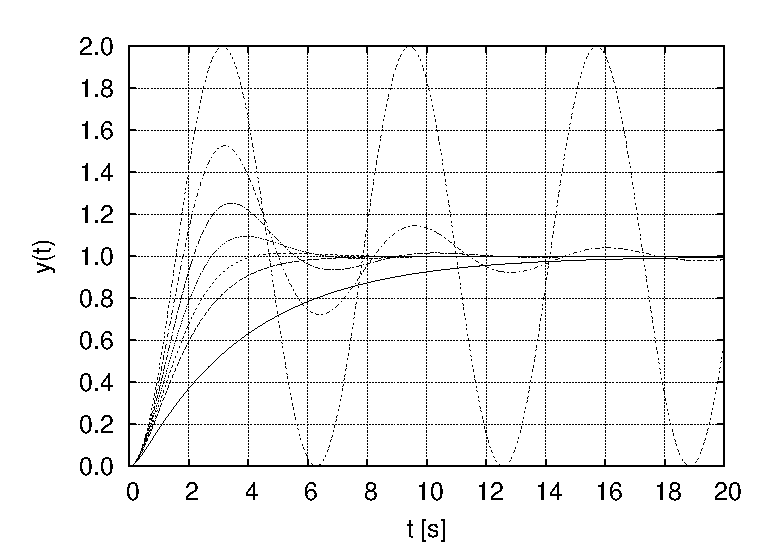
\includegraphics[width=0.8\linewidth]{fig/StepResponse.eps}
  \caption{Step response of second order systems: 
    damping coefficient affects convergence speed.}
  \label{fig:snapthru}
\end{figure}

\subsection{図の配置}
Floatingパラメータを調整してあるので,
意図した場所に入ることが多いが,
入らなかった場合には,図の大きさや位置を調整すること.


\section{図の作成に関する注意}
EPSファイルを作成する際に注意すべきは,図の種類がベクトルグラフィックスか
ビットマップグラフィックスかの違いを意識して
EPSファイルを作成することである.
グラフ・ブロック線図等は前者であり,写真は後者である.
この事を意識せずにデータを作ると,見苦しいグラフや巨大なEPSファイルを
作ることになる.
Fig.~\ref{fig:ComparingEPS}に例を示すので拡大して比較せよ.
なお,説明のためにFig.~\ref{fig:ComparingEPS}のキャプションは
日本語としてあるが,本来は英語で記載すること.
%
\begin{figure}[tb]
  \centering
  \begin{tabular}[t]{cc}
    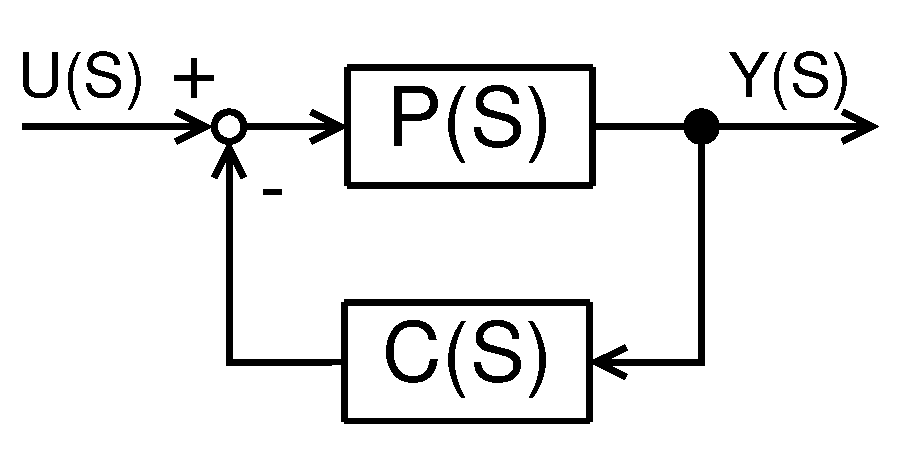
\includegraphics[width=0.65\linewidth]{fig/Feedback.eps} \\
    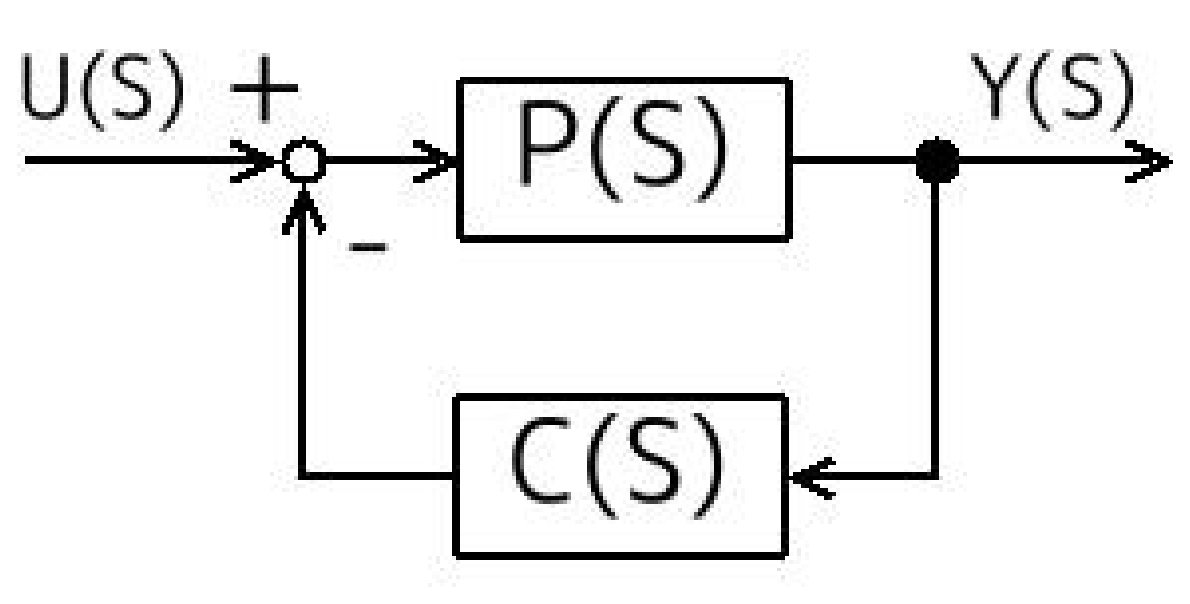
\includegraphics[width=0.65\linewidth]{fig/Feedback-jpeg.eps}
  \end{tabular}
  \caption{diaを用いてベクトルデータで作成したブロック線図:
    上はベクトルEPS,下はビットマップEPS(JPEGファイルで保存し
    jpeg2psを用いてEPSに変換).
    下図ではエイリアスが発生している.}
  \label{fig:ComparingEPS}
\end{figure}

以下では図の種類ごとにEPSファイルを作成するための指針を示す.
ツールの詳細は文献\cite{TeXWiki}の「変換ツール」を参照すること.

\subsection{グラフ}
gnuplotやExcelなどを使用して作成する.
\subsubsection{gnuplot}
gnuplotの使用法は文献\cite{GnuplotPerfect,GnuplotTP}が詳しい.
次のようにコマンド入力すると,\texttt{foo.eps}が作成される.
\begin{verbatim}
> set terminal postscript eps
> set output "foo.eps"
> replot
\end{verbatim}
EPSファイルのフォントサイズを20ポイントにする場合には,
ターミナル設定で次のようにする
\footnote{texで図をスケールするとフォントサイズも変化することに注意する}.
\begin{verbatim}
> set terminal postscript eps 20
\end{verbatim}

\subsubsection{Excel}
\texttt{wmf2eps}を利用するとExcelの図をベクトルデータのままでEPSに変換で
きて大変便利である.設定などの詳細は文献\cite{WMF2EPS}を参照する.

\subsection{ブロック線図などの図}
Fig.~\ref{fig:block}のような,
線や円を中心としたベクトルデータの図形は
OpenOffice.orgのDraw,diaや
Visio, PowerPointなどを使用して作成する.
DrawとdiaではEPSを直接作成できる.
また前述の\verb+wmf2eps+を用いると
Microsoft officeの図をEPS形式にして保存できる.
% 
\begin{figure}[tb]
  \centering
  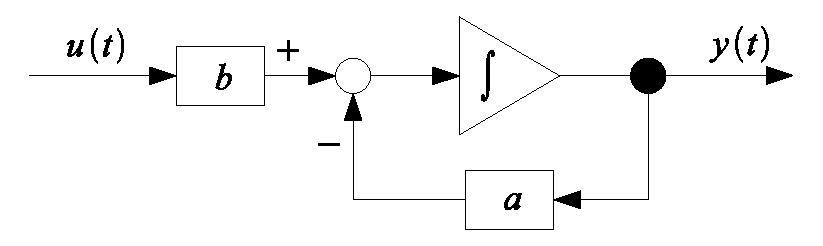
\includegraphics[width=0.9\linewidth]{fig/SFDiagram.eps}
  \caption{State flow diagram depicted with ``OpenOffice.org Draw.''}
  \label{fig:block}
\end{figure}
\subsubsection{WMF2EPS}
\verb+wmf2eps+を用いるとPowerPointなどMicrosoft office
で作成した図をコピーアンドペーストでEPS形式にして保存できるので
Windows上では大変便利なので利用を勧める\cite{WMF2EPS}.
\subsubsection{OpenOffice.org Draw}
OpenOffice.orgのDrawを用いると高品質のベクトルデータのEPSを
直接作成できる.保存する際にオブジェクトを選択し,選択範囲をEPSとして
エクスポートすればよい(\verb+http://ja.openoffice.org/+).
\subsubsection{dia}
ベクトルデータのEPSファイルを直接作成できる
(\verb+http://www.gnome.org/projects/dia/+).
\subsubsection{VisioとPowerPoint(wmf形式)}
WMF形式のファイルは,
\texttt{wmf2eps}を利用するとベクトルデータのまま
EPSに変換できる.
\subsubsection{PDF形式とAcrobatを用いた変換}
PDF形式で出力した後に,Acrobatで文字などを加えて
文書/トリミングで範囲を選択した後に
EPSファイルとして保存できる.
Visioではアドインを利用すればPDFで保存できる.
Acrobatから直接EPSを選択してdvioutがエラーを
発生する場合は,PSファイルに一度保存し,
Photoshopなどで再度EPSファイルに保存すると良い.

\subsection{写真など}
JPEGファイルは,\texttt{jpeg2ps}を用いると
画像の品質を損なうことなく,サイズもほとんど同じ
EPSファイルに変換できる.例:
\begin{verbatim}
  > jpeg2ps foo.jpg -o foo.eps
\end{verbatim}

\subsection{Linux上のツール}
tgif, xfig, diaなど,
Linuxでは\TeX やEPSなどに対応したツールが充実している.


\section{プログラムなど文字をそのまま出力する方法}
プログラムのソースなどを\TeX で表示する場合は
\verb+verbatim+環境を用いる.
\verb+\begin{verbatim}+と\verb+\end{verbatim}+の間は,
以下のように\TeX の文字が空白も含めてそのまま表示される.
\begin{verbatim}
#include <stdio.h>
int main()
{
   printf("Hello, world\n");
   return 0;
} 
\end{verbatim}


\section{書式に関する注意}
\TeX による文書作成において,改段落の方法の誤りをよく目にする.
日本語の文章では文章の区切りで改行し,
新しい行の先頭は全角一文字分の空白を入れる.
たとえば,この文を段落の終わりとする.

次の段落はこのように始まる.\LaTeXe でこれを実現するには,
\texttt{tex}ファイルに改行命令\verb+\\+を入れるのではなく,
ただ改行し,空行を入れて,先頭に1文字分の空白を入れずに
次の段落の文章を始めればよい.
なお,\verb+\section+コマンドの後の文章は段落の
始まりと考えられるので,行の先頭に自動的に空白が入る.

そのほかに下記に注意する.
\begin{itemize}
\item 文章中の数字は全角ではなく半角で記述する.
  例えば``2006年''ではなく``2006年''とする.
\item 句点:``。``ではなく''.``を用いる.
\item 読点:``、``ではなく'',``を用いる.
\end{itemize}

{\small
\begin{thebibliography}{99}
\bibitem{msetemplateB}
  (2011, Jan. 23) 機械システム工学科:
  ``卒業論文概要原稿の書き方'',東京都市大学~工学部.[Online].
  Available: \url{http://www.mse.tcu.ac.jp/defense.html}
\bibitem{Okumura2000}
  奥村晴彦:
  ``改訂版\LaTeXe 美文書作成入門'',
  技術評論社,2000.
\bibitem{LaTeXeBook}
  中野賢:
  ``日本語\LaTeXe ブック'',
  アスキー出版局,1996.
\bibitem{GnuplotPerfect}
  川原稔:
  ``Gnuplot パーフェクトマニュアル'',
  Soft Bank, 1999.
\bibitem{GnuplotTP}
  矢吹道郎,大竹敢:
  ``使いこなすGnuplot'',
  Techno Press, 2000.
\bibitem{Kagi}
  (2009, Dec. 7) 物理のかぎしっぽ.[Online].
  Available: \url{http://hooktail.org/computer/index.php?TeX}
\bibitem{TeXWiki}
  (2009, Dec. 7) \TeX \texttt{Wiki}. [Online].
  Available: \url{http://oku.edu.mie-u.ac.jp/~okumura/texwiki/}
\bibitem{texinstaller}
  (2009, Dec. 7) TeXインストーラ3のダウンロード.[Online].
  Available: \url{http://www.ms.u-tokyo.ac.jp/~abenori/mycreate/index.html}
\bibitem{WMF2EPS}
  (2009, Dec. 7) TeXに張り付けるEPS形式の図をWindows上で作成する方法.[Online].
  Available: \url{http://www.mtl.t.u-tokyo.ac.jp/~iizuka/nt/eps/}
\end{thebibliography}
}

\section*{謝辞}
初版から2.4版まで作成してくださった野中謙一郎先生に感謝します.


\appendix
\section{更新履歴}
%%最終更新 \today\\
\begin{tabular}[t]{|l|l|l|} \hline
  版 & 更新日 & 備考 \\ \hline \hline
  1.0 & 2001/12/15 & 初版 \\ \hline
  1.1 & 2001/12/25 & 数学記号を追記 \\ \hline
  1.2 & 2001/12/28 & \verb+\section+フォント修正 \\
  & & \verb+\figurewidth+を設定 \\ \hline\hline
  2.0 & 2007/01/07 & 2006年度版に対応 \\
  & & 最近のソフトウエアを紹介 \\
  & & 研究室名の改行を防止 \\
  & & 図のキャプションの空白を短縮 \\
  & & 1節の見出し前の空行を削除 \\ \hline
  2.1 & 2007/01/10 & 図の空白を調整 \\
  & & グラフを入れ替え \\
  & & 1節の見出しのフォントを修正 \\ \hline
  2.2 & 2008/05/05 & DrawとPDFによる作図を加筆 \\ \hline
  2.3 & 2008/06/12 & TeXインストーラplug-inを加筆 \\ \hline
  2.4 & 2009/12/07 & \verb+wmf2eps+について詳しく追記 \\
  & & \verb+verbatim+環境を追加 \\ \hline\hline
  3.0 & 2011/08/25 & 2011年度版に改訂 \\ \hline
  3.1 & 2015/08/24 & Abstract, Key words, Referenceを9pt(small)にした \\ \hline
\end{tabular}

\end{document}

%%% Local Variables: 
%%% End: 
